% report.tex — Отчёт по преддипломной практике
% Пронина А.И., ИТМО, 2026

\documentclass{itmo-vkr}

\usepackage{xcolor}

% Разрешить перенос URL по слешам и точкам
\makeatletter
\g@addto@macro\UrlBreaks{\do\/\do-\do.\do_}
\makeatother
\usepackage{float}
\usepackage{graphicx}
\graphicspath{{figures/}}
\usepackage{pdfpages}

\title{Отчёт по преддипломной практике}
\author{Пронина А.~И.}
\date{2026}

\begin{document}

% ===== ТИТУЛЬНЫЙ ЛИСТ =====
\begin{titlepage}
\thispagestyle{empty}

\begin{center}
    Министерство науки и высшего образования Российской Федерации\\[0.3cm]
    федеральное государственное автономное образовательное учреждение высшего образования\\[0.3cm]
    «Национальный исследовательский университет ИТМО»\\[0.2cm]
    (Университет ИТМО)
\end{center}

\vspace{0.8cm}

\begin{center}
    Факультет программной инженерии и компьютерной техники\\[0.1cm]
    Образовательная программа: Компьютерные системы и технологии\\[0.1cm]
    Направление подготовки (специальность): 09.03.01~-- Информатика и вычислительная техника\\[0.1cm]
\end{center}

\vspace{1.2cm}

\begin{center}
    {\Large \textbf{О Т Ч Ё Т}}\\[0.6cm]
    о производственной, преддипломной практике\\[0.6cm]
    Тема задания: \textbf{«Разработка инструмента планирования миграции кодовой базы проекта на алгоритмы постквантовой криптографии»}
\end{center}

\vspace{1.5cm}

Обучающийся: Пронина Анастасия Ильинична

№ группы: Р3433

\noindent\hspace{1.2cm}\begin{minipage}[t]{\dimexpr\textwidth-1.5cm}
    Руководитель практики от университета:\\
    Рыбаков Степан Дмитриевич, преподаватель практики
\end{minipage}

\hfill 26.05.2026

\vfill

\begin{center}
    Санкт-Петербург\\
    2026~г.
\end{center}

\end{titlepage}

% ===== СОДЕРЖАНИЕ =====
\tableofcontents
\newpage

% ===== ВВЕДЕНИЕ =====
\unnumberedchapter{ВВЕДЕНИЕ}

Производственная, преддипломная практика является заключительным этапом подготовки к защите выпускной квалификационной работы. Настоящая практика проходила на факультете программной инженерии и компьютерной техники Университета ИТМО под руководством Рыбакова Степана Дмитриевича в период с 30~апреля по 28~мая 2026~года.

Целью практики являлось написание и оформление текста ВКР на тему «Разработка инструмента планирования миграции кодовой базы проекта на алгоритмы постквантовой криптографии», проверка текста на оригинальность, а также представление результатов работы на предзащите.

Перед началом практики я поставила перед собой следующие задачи:

\begin{enumerate}
    \item завершить написание и оформление текста ВКР в соответствии с нормами Университета ИТМО;
    \item пройти проверку текста через систему «Антиплагиат» и получить справку с результатами;
    \item подготовить презентацию для предзащиты и пройти предзащиту с оценкой готовности не ниже 70\%;
    \item составить и оформить настоящий отчёт о прохождении практики.
\end{enumerate}

Перечень этапов практики и их содержание представлены в таблице~\ref{tab:stages}.

\begin{longtable}{|>{\centering\arraybackslash}p{0.6cm}|p{3.8cm}|>{\centering\arraybackslash}p{1.8cm}|p{8.3cm}|}
    \caption{Этапы преддипломной практики} \label{tab:stages} \\
    \hline
    № & Название этапа & Период, дн. & Содержание задания \\ \hline
    \endfirsthead
    \multicolumn{4}{r}{\textit{Продолжение таблицы \thetable}} \\ \hline
    № & Название этапа & Период, дн. & Содержание задания \\ \hline
    \endhead
    \hline
    \endlastfoot

    1 & Инструктаж обучающегося & 1
      & Инструктаж обучающегося по ознакомлению с требованиями охраны труда, техники безопасности, пожарной безопасности, а также правилами внутреннего трудового распорядка. \\ \hline

    2 & Написание текста ВКР & 15
      & {\small Подготовить текст ВКР в соответствии с инд. заданием. Текст ВКР представляется в электронном виде и включает введение, основную часть, заключение (не менее 40 страниц, в которые не входят титульный лист, аннотация, задание на ВКР, оглавление/содержание, список сокращений, список источников и приложения). Во введении дается общая характеристика работы (актуальность темы, цель и задачи, степень проработанности проблемы, практическая значимость работы, апробация и внедрение результатов исследования, личный вклад). При составлении обзора необходимо использовать не менее 20 источников не старше 5 лет, в том числе не менее 20\% научных статей в изданиях, рекомендованных ВАК РФ для диссертаций, и не менее 15\% в изданиях, индексируемых в базах WoS/Scopus. В заключении приводится список основных результатов исследования, с обоснованием их научной и практической значимости. При формулировке результатов необходимо указывать количественные и качественные характеристики экспериментальных исследований, подтверждающих достижение поставленной цели. Обязательным пунктом заключения должны быть пути дальнейших направлений исследований по теме ВКР. К отчёту текст ВКР не прикладывается. \\ \hline

    3 & Проверка текста ВКР в системе «Антиплагиат» & 6
      & Сдать на проверку текст ВКР секретарю ГЭК и получить справку о прохождении проверки (оригинальность не менее 75 процентов или не более 25\% заимствований). В отчёт в приложении поместить полученную справку. \\ \hline

    4 & Предзащита ВКР & 8
      & Подготовить электронную презентацию (не более 15 слайдов) с результатами работы и пройти предзащиту (готовность к защите не менее 70\%). В отчёт в приложении поместить презентацию. \\ \hline

    5 & Оформление отчёта & 28
      & Написание отчёта, оформление в соответствии с требованиями, получение отзыва от руководителей. Оформление отчётных документов в соответствии с требованиями: 1.~Оформление отчёта должно быть выполнено в соответствии с методическим пособием (\url{https://books.ifmo.ru/file/pdf/2622.pdf}), за исключением структуры. 2.~Структура документа: титульный лист, введение, основная часть, заключение, приложения. 3.~В основной части подробно описывается выполнение задач 2--4 этапов. \\ \hline

    6 & Получение отзыва с оценкой от руководителя & 1
      & Получить отзыв с оценкой у руководителя практики в модуле «Практика». \\

\end{longtable}

К началу преддипломной практики программная часть проекта~-- инструмент на C++17 для автоматической инвентаризации квантово-уязвимых криптографических вызовов в C/C++-коде~-- была уже реализована и протестирована. Содержанием практики стало оформление полученных результатов: написание текста ВКР, работа с источниками, подготовка иллюстративного материала, приведение текста в соответствие с требованиями Университета ИТМО, а также подготовка к предзащите.

\newpage

% ===== ОСНОВНАЯ ЧАСТЬ =====
\section{Написание текста ВКР}

Работа над текстом ВКР заняла основной период практики: с 30~апреля по 14~мая~2026~года. К этому моменту проект был уже реализован и протестирован; задача этапа состояла в том, чтобы грамотно изложить всю проделанную работу в виде законченного текста объёмом не менее 40 страниц.

\subsection{Формирование структуры ВКР}

Работу над текстом ВКР я выстраивала по принципу «обзор темы~-- описание инструмента»: сначала изложить теоретическую базу, обосновать актуальность задачи и рассмотреть существующие аналоги, а затем последовательно описать разработанное решение. Первоначально я начала первый раздел непосредственно с квантовых угроз и алгоритма Шора. Однако в ходе обсуждения с руководителем~-- Рыбаковым Степаном Дмитриевичем~-- он предложил предварить эту часть отдельным подразделом об основах современной криптографии: симметричных и асимметричных алгоритмах, цифровой подписи и инфраструктуре открытых ключей~-- чтобы читателю было понятно, что именно взламывается квантовым компьютером и почему это критично. Я приняла это предложение, и в итоговой структуре этот подраздел открывает первую главу.

Дальнейшую структуру я выстраивала по мере написания: каждому модулю инструмента и этапу тестирования я посвятила отдельный раздел. В итоге работа сложилась в шесть разделов: анализ угроз и нормативной базы, обзор аналогов, проектирование архитектуры, реализация, тестирование и оценка, анализ полученных результатов.

Текст я писала в~\LaTeX{}, используя шаблон ИТМО, разработанный мною в ходе учебной практики. Документ включает: оглавление, список сокращений и условных обозначений, список терминов и определений, введение, шесть основных разделов, заключение, список использованных источников (более 50 позиций) и приложения. Работу я начала с теоретической части, поскольку она задаёт понятийную базу для остальных разделов, и завершила введением и заключением~-- когда структура и содержание работы были полностью сформированы.

\subsection{Работа с источниками}

Поиск источников я вела по мере продвижения по разделам, подбирая материал под конкретные подтемы. Для русскоязычных публикаций использовались платформы eLIBRARY и «КиберЛенинка» с ориентацией на журналы из перечней ВАК и Scopus; для англоязычных~-- базы IEEE Xplore и ACM Digital Library. Нормативные документы я искала напрямую на сайтах NIST и ТК~26. Поисковые запросы строились по ключевым темам каждого подраздела: «постквантовая криптография», «алгоритм Шора», «квантовые угрозы криптографии», «стандарты NIST PQC», «криптографическая миграция», «статический анализ кода». Приоритет отдавался публикациям не старше 5 лет; для исторически значимых работ привлекались первоисточники (например, оригинальная статья Шора 1994~года).

Итоговый список источников, который я сформировала, насчитывает более 50 позиций и охватывает официальные документы NIST (FIPS~203, FIPS~204, FIPS~205, NIST~IR~8547), аналитические доклады Global Risk Institute и Project Eleven, техническую документацию Google Quantum AI и IBM, статьи из баз IEEE и ACM, российские нормативные документы ТК~26 и открытые спецификации CycloneDX.

Среди изученных источников я выделила два как опорных для обоснования актуальности. Статья Крейга Гидни (2025) содержит пересмотренные оценки ресурсов, необходимых для взлома RSA-2048: менее одного миллиона физических кубитов и менее недели времени~-- в 20 раз эффективнее оценок того же автора 2019~года. Совместный доклад IBM Institute for Business Value и Cloud Security Alliance (2025) фиксирует, что лишь около 30\% организаций завершили криптографическую инвентаризацию своих систем.

Все источники по мере изучения я добавляла в файл \texttt{references.bib} и оформляла с помощью BibLaTeX в стиле GOST-numeric, с сортировкой по порядку появления в тексте.

\subsection{Написание основных разделов}

\textbf{Первый раздел (теоретический).} Я начала с изложения основ криптографии, необходимых для понимания квантовой угрозы: симметричные и асимметричные алгоритмы, цифровая подпись, инфраструктура открытых ключей. Затем описала алгоритм Шора и алгоритм Гровера с пояснением их практического значения: именно это разграничение объясняет, почему RSA, ECDSA и DH вошли в базу уязвимых функций, а AES-256 и «Кузнечик»~-- нет. Отдельно описала стандарты NIST FIPS~203/204/205 и российскую ситуацию: алгоритмы-кандидаты ТК~26 («Шиповник», «Гиперикум», «Кодиеум») и их нынешний статус. Написание этой части потребовало наибольшей проработки источников.

\textbf{Второй раздел (анализ аналогов).} Я рассмотрела семь инструментов: IBM Quantum Safe Explorer, CodeQL, CBOMkit, CryptoScan, SonarQube, CycloneDX~cdxgen и предложения QApp. Для каждого зафиксировала поддержку C/C++, наличие оценки квантового риска, поддержку ТК~26 и NIST IR~8547. Написание этого раздела потребовало аккуратного изложения: важно было не просто перечислить ограничения аналогов, но и показать, какое именно место на карте инструментов занимает разработанное решение.

\textbf{Третий раздел (проектирование).} Здесь я описала архитектурные решения: выбор конвейерной модели, обоснование модульной структуры и хранения базы во внешнем JSON-файле, описание структур данных (Finding, CertInfo, RiskScore, MigrationAction, Cbom) и полную спецификацию функциональных и нефункциональных требований.

\textbf{Четвёртый раздел (реализация и тестирование).} Описала работу каждого программного модуля: от инвентаризации проекта до генерации CBOM. Отдельное внимание уделила AST-анализатору как наиболее сложному компоненту: многоуровневой трассировке аргументов, построению графа вызовов через BFS и механизму подавления находок. В раздел тестирования я включила описание тестовых данных, методику оценки метрик precision/recall/F1, анализ причин ложных срабатываний и ограничения реализации.

\subsection{Введение, заключение и оформление}

Введение и заключение я написала в последнюю очередь~-- когда структура и содержание работы были окончательно сформированы. Во введении я сформулировала актуальность, цель и пять задач, соответствующих разделам основной части. В заключении зафиксировала выполнение каждой задачи и подвела количественный итог: показатели точности анализаторов, число тестов, результаты запуска инструмента на реальном проекте.

Я подготовила рисунки (архитектурные схемы, диаграммы последовательности, примеры JSON-вывода), вставила листинги кода и расставила перекрёстные ссылки на рисунки, таблицы и формулы.

Параллельно с написанием текста я формировала список сокращений и условных обозначений и список терминов и определений. Сокращения я вносила по мере появления; итоговый список я упорядочила по алфавиту. Определения терминов я составляла на основе изученных источников; они охватывают ключевые понятия предметной области: квантовый компьютер, постквантовая криптография, CBOM, криптографическая инвентаризация и ряд других. Особое внимание я уделила единообразию обозначений: все сокращения (CRQC, HNDL, PQC, ML-KEM) расшифрованы при первом упоминании и используются единообразно на протяжении всего документа.

\subsection{Итерации с руководителем}

В процессе написания я дважды направляла текст руководителю на проверку.

После первой итерации~-- когда были готовы первые две главы (анализ квантовых угроз и нормативной базы, анализ аналогов)~-- руководитель высказал три замечания. Во-первых, он рекомендовал расширить подраздел об основах современной криптографии: материал о симметричных и асимметричных алгоритмах был изложен недостаточно подробно, чтобы служить полноценной точкой входа для читателя; я дополнила подраздел описанием гибридного шифрования, цифровой подписи и инфраструктуры открытых ключей. Во-вторых, руководитель указал на необходимость подкреплять каждый приводимый факт ссылкой на источник: утверждения о сроках появления квантового компьютера, статистика готовности отрасли, оценки вычислительных ресурсов~-- всё это требует конкретных ссылок, а не общих отсылок к «мировой практике»; по итогам правки я добавила ссылку на первоисточник к каждому количественному утверждению. В-третьих, руководитель обратил внимание на стиль изложения: в тексте встречались излишне экспрессивные формулировки и широкие обобщения, не характерные для формализованного текста; подобные места я переработала в пользу нейтрального стиля.

Вторая итерация охватила готовый текст целиком. Замечания затронули несколько аспектов. В ряде листингов на странице оставалась одна строка кода или только подпись; я добавила в шаблон ограничение на минимальное количество строк листинга на странице. Кроме того, из-за переноса таблиц и рисунков на следующие страницы в тексте образовывались большие пустые области; я скорректировала оформление так, чтобы свободное пространство распределялось равномерно. На ряде рисунков стрелки на диаграммах сместились относительно блоков; я перерисовала диаграммы. Наконец, руководитель обратил внимание на отсутствие лицензии в публичном репозитории на GitHub; я добавила лицензию Apache 2.0. По итогам этой итерации я сдала текст на нормоконтроль.

\newpage

\section{Проверка текста ВКР в системе «Антиплагиат»}

\subsection{Процедура проверки}

Процедура проверки состояла из двух этапов.

\textbf{Этап~1~-- Нормоконтроль и передача секретарю ГЭК.} Перед загрузкой в систему я направила готовый текст ВКР своему секретарю ГЭК~-- Смирновой Анжелике Леонидовне~-- для прохождения нормоконтроля. На этом шаге проверялось соответствие оформления документа требованиям: структура разделов, оформление списков и таблиц, правильность оформления ссылок и списка источников.

По результатам нормоконтроля я получила два замечания:
\begin{enumerate}
    \item \textit{Ссылки на все листинги и рисунки.} Секретарь указала на необходимость убедиться, что в тексте есть явная ссылка на каждый рисунок и каждый листинг кода~-- иначе они считаются «висячими» элементами, не связанными с основным текстом. Я проверила весь документ и добавила недостающие ссылки.
    \item \textit{Стиль заголовка «Содержание».} Секретарь указала, что заголовок раздела «Содержание» должен быть оформлен в том же стиле, что и все остальные структурные заголовки ВКР. Я устранила замечание, исправив соответствующую настройку в шаблоне.
\end{enumerate}

После устранения замечаний секретарь подтвердила готовность текста к загрузке в систему.

\textbf{Этап~2~-- Загрузка в my.itmo и проверка.} Подготовленный текст я самостоятельно загрузила через личный кабинет на портале my.itmo. Там документ был автоматически направлен на проверку в систему «Антиплагиат». В ходе проверки использовался расширенный набор модулей поиска, в том числе:
\begin{itemize}
    \item базы научных публикаций~-- IEEE, PubMed, eLIBRARY, РГБ, сводная коллекция ЭБС;
    \item российские нормативно-правовые базы~-- СПС ГАРАНТ;
    \item интернет-коллекции и специализированные базы~-- СМИ России и СНГ, Рувики, коллекция НБУ, Кольцо вузов;
    \item модули перефразирований и переводных заимствований по коллекциям IEEE, PubMed, eLIBRARY и интернет-сегменту.
\end{itemize}

\subsection{Результаты проверки}

Проверка была выполнена 20~мая~2026~года. Итоговые показатели по справке системы «Антиплагиат» представлены в таблице~\ref{tab:antiplagiat}.

\begin{table}[h]
    \caption{Результаты проверки текста ВКР на заимствования}
    \label{tab:antiplagiat}
    \begin{tabular}{|p{7cm}|r|}
        \hline
        Показатель & Значение \\ \hline
        Оригинальность & 97,49\% \\ \hline
        Совпадения & 2,51\% \\ \hline
        Цитирования & 0\% \\ \hline
        Самоцитирования & 0\% \\ \hline
        ИИ-контент & 0\% \\ \hline
        Дата проверки & 20.05.2026 \\ \hline
        Работу проверил & Смирнова А.~Л. \\ \hline
    \end{tabular}
\end{table}

Полученный уровень оригинальности~(97,49\%) значительно превышает установленный минимальный порог для программ бакалавриата~(75\%). Совпадения~(2,51\%) приходятся преимущественно на общепринятую терминологию предметной области: названия алгоритмов (RSA, ECDSA, ML-KEM), стандартов (FIPS~203, NIST IR~8547) и устойчивые профессиональные словосочетания, неизбежно присутствующие в любой работе по данной тематике. Нулевой показатель ИИ-контента подтверждает самостоятельное написание текста.

Справка о результатах проверки предоставлена в качестве \hyperref[app:A]{Приложения~А}.

\newpage

\section{Предзащита ВКР}

На данном этапе мне предстояло подготовить электронную презентацию и речь к ней, после чего пройти предзащиту в формате видеоконференции.

\subsection{Подготовка презентации}

Презентацию я составила на основе ключевых результатов ВКР. В ней 14~слайдов со следующей структурой:

\begin{enumerate}
    \item \textbf{Слайд~1 -- Титульный.} Тема, студент (Пронина А.~И., гр.~Р3433), руководитель (Рыбаков~С.~Д.).
    \item \textbf{Слайд~2 -- Актуальность: квантовая угроза и сроки.} Перечень алгоритмов, уязвимых к алгоритму Шора (RSA, DSA, DH, ECDH, ECDSA, ГОСТ~Р~34.10-2012), прогнозы появления криптографически значимого квантового компьютера (CRQC): Global Risk Institute~-- 28--49\% в ближайшие 10~лет, Project~Eleven~-- Q-Day~$\approx$~2033. Временная шкала нормативных событий: публикация NIST FIPS~203/204/205 (2024), устаревание RSA-2048 и ECDSA~P-256 (2030), Q-Day (2033), полный запрет квантово-уязвимых алгоритмов (2035).
    \item \textbf{Слайд~3 -- Актуальность: инвентаризация и срочность.} Масштаб проблемы в C/C++-коде, данные IBM IBV и CSA (2025) о готовности отрасли (30\% организаций завершили инвентаризацию, 24\% применяют результаты), угроза HNDL («Harvest Now, Decrypt Later» -- перехват зашифрованного трафика уже сейчас с целью расшифровки после появления CRQC).
    \item \textbf{Слайд~4 -- Цель и задачи.} Формулировка цели и пяти задач работы.
    \item \textbf{Слайд~5 -- Анализ аналогов.} Сравнительная таблица 7 инструментов (IBM Quantum Safe Explorer, CodeQL, CBOMkit, CryptoScan, SonarQube, cdxgen, QApp) по критериям: поддержка C/C++, ТК~26/ГОСТ, план миграции, NIST IR~8547. Вывод: ни один не реализует полноценной цепочки.
    \item \textbf{Слайд~6 -- Архитектура: модульный конвейер.} Компонентная схема системы с потоками данных между модулями Configuration~Manager, Signature~DB, Project~Scanner, Regex~Analyzer, AST~Analyzer, Cert~Analyzer, Risk~Assessor, Report~Generator.
    \item \textbf{Слайд~7 -- Архитектура: процесс выполнения.} Временная диаграмма взаимодействия всех компонентов (sequence diagram).
    \item \textbf{Слайд~8 -- Пример работы: ГОСТ-функция в коде.} Входной фрагмент с вызовом \texttt{EVP\_PKEY\_CTX\_new\_id} через ГОСТ-идентификатор, соответствующий фрагмент JSON-отчёта. На примере показана работа механизма разрешения аргументов: инструмент корректно отличает уязвимый вызов от вызова с постквантовым аргументом.
    \item \textbf{Слайд~9 -- Пример работы: отчёт о плане миграции.} Фрагменты трёх секций JSON-отчёта: сводка по файлу, запись плана замены функции, информация о сертификате.
    \item \textbf{Слайд~10 -- Демонстрация работы.} Скриншот рабочего окружения: структура проекта в VSCode и примеры команд запуска инструмента в базовом, AST и метрическом режимах.
    \item \textbf{Слайд~11 -- Практический результат: экономия времени.} Задача: криптографическая инвентаризация проекта из 23~файлов C/C++ ($\approx$7000~строк). Найдено 573~вызова криптографических функций, из них 44~квантово-уязвимых. Сравнение: ручной поиск~-- $\approx$18--20~часов, утилита~-- $\approx$1~с. (regex) / $\approx$13~с. (AST). Ускорение~$\geq 5 \cdot 10^3$ раз.
    \item \textbf{Слайд~12 -- Метрики качества: AST vs Regex.} Таблица с TP/FP/FN, precision/recall/F1 и временем анализа для обоих режимов. Пояснение причин преимущества AST-режима и анализ оставшихся ложных срабатываний.
    \item \textbf{Слайд~13 -- Результаты работы.} Сводный список результатов, подтверждение выполнения всех пяти задач и достижения цели.
    \item \textbf{Слайд~14 -- Благодарность и ссылка.} Ссылка на публичный репозиторий с исходным кодом инструмента.
\end{enumerate}

Параллельно с подготовкой слайдов я составила речь к докладу и провела несколько репетиций с замером времени, чтобы уложиться в отведённый регламент.

Презентация включена в настоящий отчёт в качестве \hyperref[app:B]{Приложения~Б}.

\subsection{Прохождение предзащиты}

Предзащита состоялась \textbf{22~мая~2026~года в 14:00} в формате видеоконференции через систему Контур.Толк. Я подключилась к конференции, дождалась своей очереди и выступила с докладом по подготовленной презентации.

\begin{figure}[H]
    \centering
    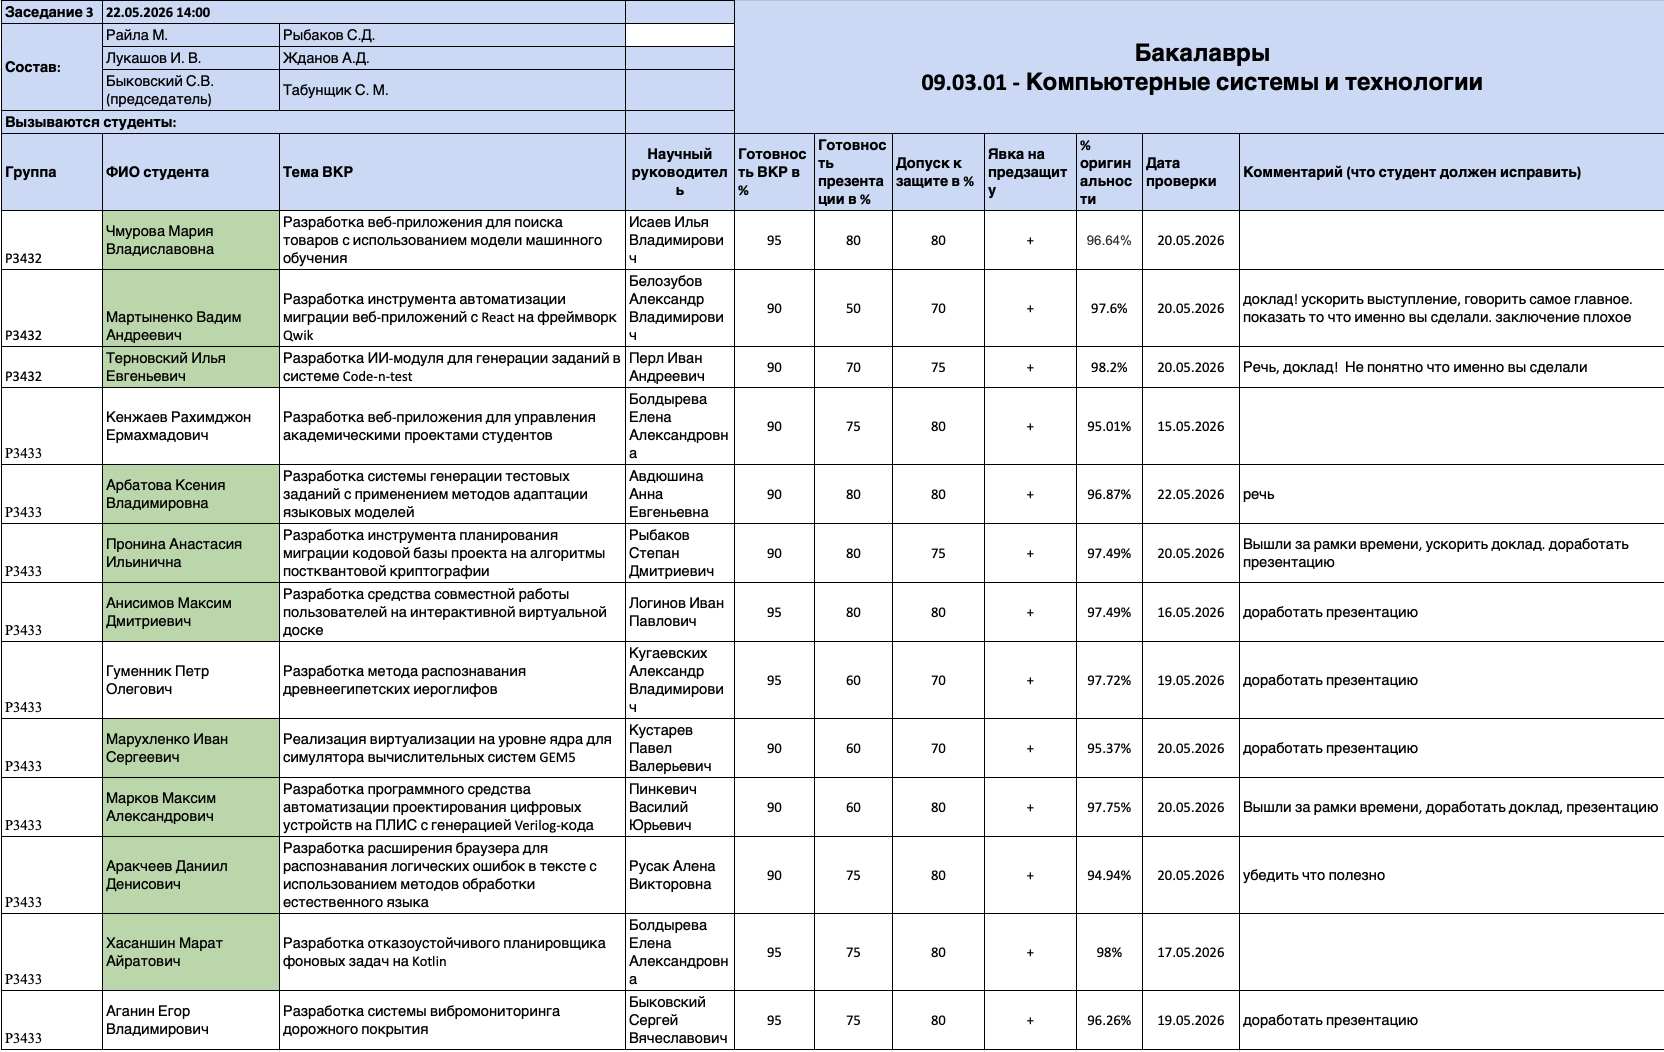
\includegraphics[width=\textwidth]{predz_screenshot.png}
    \caption{Таблица результатов участия в предзащите ВКР (22.05.2026)}
\end{figure}

\textbf{Превышение регламента.} В ходе доклада я вышла за отведённое время примерно на~1,5~минуты. На это мне указали члены комиссии. Причиной стало недостаточно жёсткое следование плану речи в моменты, когда я отступала от подготовленного текста.

\textbf{Вопросы и замечания комиссии.} По итогам доклада члены комиссии задали вопросы и высказали замечания; ниже каждый из них приводится с моим ответом.

\begin{enumerate}
    \item \textit{Вопрос: на каком основании разным алгоритмам присваиваются разные базовые оценки риска?} Я пояснила, что оценка зависит от степени уязвимости к квантовым атакам: асимметричные алгоритмы (RSA, ECDSA, DH и др.) получают максимальную оценку, так как полностью компрометируются алгоритмом Шора; симметричные алгоритмы с короткими ключами и устаревшие хеш-функции получают пониженную, но ненулевую оценку. Комиссия приняла ответ.

    \item \textit{Замечание: масштаб временной шкалы на слайде~11 некорректен.} Ось времени на слайде с практическим результатом построена до~14~часов, тогда как ручной поиск занимает~18--20~часов, из-за чего правый столбец диаграммы выходит за её пределы. Я признала замечание обоснованным и ответила, что при доработке расширю шкалу до 20~часов.

    \item \textit{Вопрос: учтено ли в сравнении время на ручную валидацию результатов инструмента?} Мне указали, что при ручном поиске аналитик верифицирует каждую находку немедленно, тогда как при автоматическом обнаружении после работы инструмента всё равно требуется ручная проверка корректности найденных уязвимостей и применимости рекомендаций. Я согласилась с тем, что это важный методологический момент, который делает сравнение некорректным, и ответила, что при доработке презентации добавлю оценку времени валидации в соответствующий слайд.

    \item \textit{Вопрос: каким образом инструмент определяет уязвимость функции~-- на основании её имени или параметров?} Я пояснила, что в инструменте реализованы два принципиально разных подхода. Regex-анализатор ищет вызовы по шаблону: он сопоставляет строки исходного кода с регулярными выражениями из базы сигнатур и не анализирует значения передаваемых аргументов. AST-анализатор, напротив, трассирует аргументы: он строит граф вызовов и отслеживает, какое значение передаётся в функцию через историю локальных переменных и привязки параметров~-- именно это позволяет отличить уязвимый вызов от вызова с постквантовым аргументом. Комиссия рекомендовала добавить это пояснение в презентацию.

\end{enumerate}

\textbf{Оценка готовности.} По итогам предзащиты комиссия выставила следующие оценки:
\begin{itemize}
    \item готовность ВКР к защите~-- 90\%;
    \item готовность презентации~-- 80\%;
    \item допуск к защите~-- 75\%.
\end{itemize}

Все показатели превышают установленный минимальный порог в 70\%.

\subsection{Обсуждение результатов с руководителем}

После предзащиты состоялось отдельное обсуждение с руководителем~-- Рыбаковым Степаном Дмитриевичем~-- по итогам выступления. Мы обсудили доработку презентации и речи к защите ВКР.

Руководитель обратил внимание на то, что в презентации не поясняется, что именно обозначает маркировка ГОСТ. Я согласилась с необходимостью при первом упоминании добавить пояснение: российские криптографические стандарты обозначаются именно так, а ГОСТ~Р~34.10-2012~-- это российский стандарт электронной цифровой подписи, уязвимый к алгоритму Шора аналогично ECDSA.

Руководитель также обратил внимание на перегруженность ряда слайдов текстом: при устном докладе это затрудняет восприятие. Я согласилась с тем, что со слайдов нужно убрать факты, которые и так звучат в речи~-- слайд должен дополнять доклад, а не дублировать его. Кроме того, мы обсудили расположение элементов на отдельных слайдах: я отметила блоки, требующие перестановки.

По поводу речи руководитель рекомендовал мне сделать более чёткий акцент на двух режимах анализа~-- AST и regex~-- как ключевом техническом вкладе работы: именно разница в подходах и показателях качества между ними наглядно демонстрирует преимущество разработанного инструмента. Все полученные рекомендации я зафиксировала для последующей доработки.

\newpage

% ===== ЗАКЛЮЧЕНИЕ =====
\unnumberedchapter{ЗАКЛЮЧЕНИЕ}

В ходе производственной, преддипломной практики я выполнила поставленную цель и все задачи в полном объёме.

На этапе написания текста ВКР я подготовила текст объёмом более 40~страниц. В его состав вошли введение, шесть основных разделов, заключение, список сокращений и условных обозначений, список терминов и определений, а также список использованных источников (более 50~позиций). Текст оформлен в соответствии с требованиями Университета ИТМО и прошёл нормоконтроль.

На этапе проверки оригинальности я передала текст на официальную проверку в систему «Антиплагиат»: оригинальность составила 97,49\% при пороге 75\% для программ бакалавриата. Справка о результатах проверки получена и приложена к настоящему отчёту.

На этапе предзащиты я подготовила электронную презентацию из 14~слайдов и речь к ней, после чего прошла предзащиту 22~мая~2026~года: комиссия оценила готовность ВКР в~90\%, готовность презентации в~80\%, допуск к защите~-- 75\%. По итогам обсуждения с руководителем я получила рекомендации по доработке презентации и речи.

Я составила настоящий отчёт в соответствии с требованиями методического пособия; он отражает ход и результаты прохождения практики.

\newpage

% ===== ПРИЛОЖЕНИЕ А =====
\appendixletter{А}
\label{app:A}
\centerline{\bfseries Справка о прохождении проверки в системе «Антиплагиат»}
\vspace{6pt}

\begin{figure}[H]
    \centering
    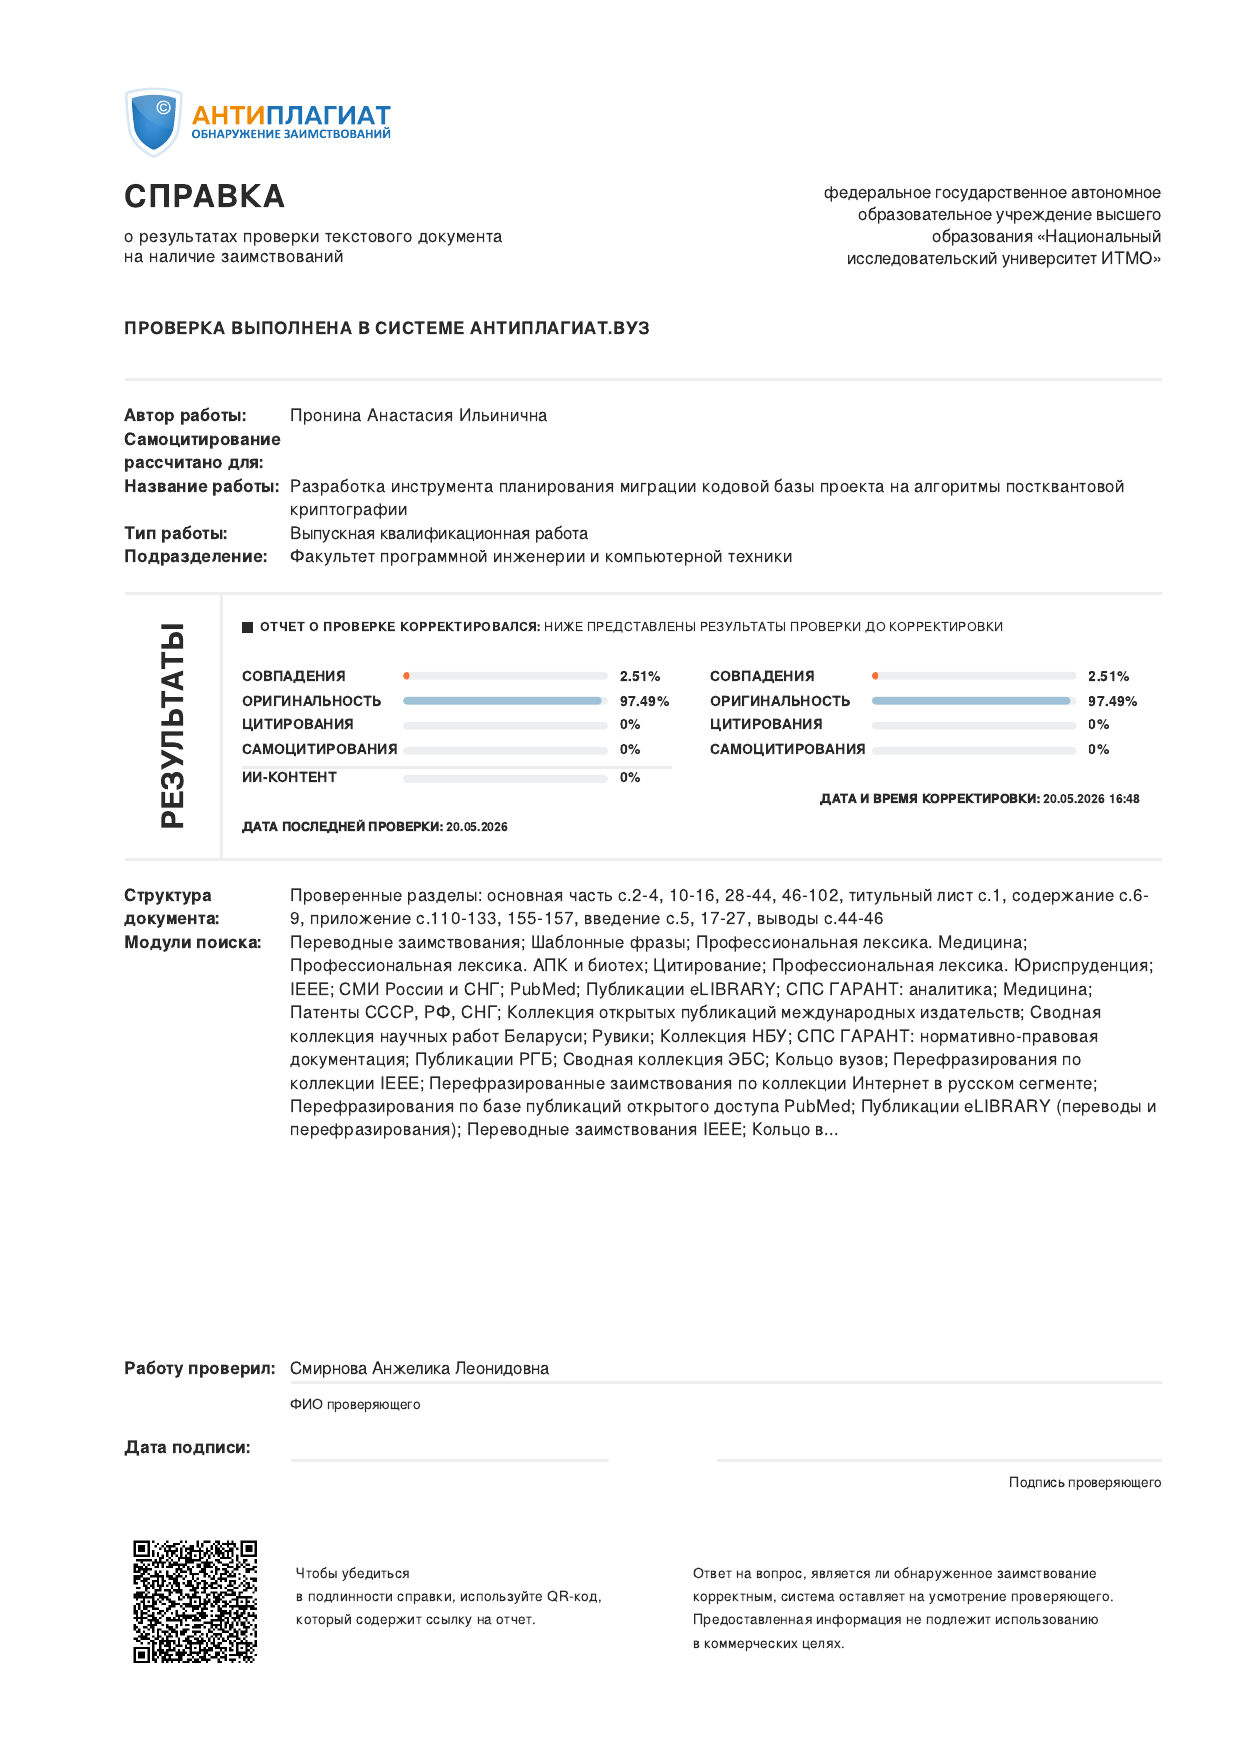
\includegraphics[width=0.85\textwidth]{antiplagiat-1.png}
    \caption{Справка о результатах проверки текста ВКР в системе «Антиплагиат»}
\end{figure}

\newpage

% ===== ПРИЛОЖЕНИЕ Б =====
\appendixletter{Б}
\label{app:B}
\centerline{\bfseries Электронная презентация к предзащите ВКР}
\vspace{6pt}

\begin{figure}[H]
    \centering
    
\includegraphics[width=\textwidth]{slides/slide-01.png}
    \caption{Слайд 1~-- Титульный}
\end{figure}

\begin{figure}[H]
    \centering
    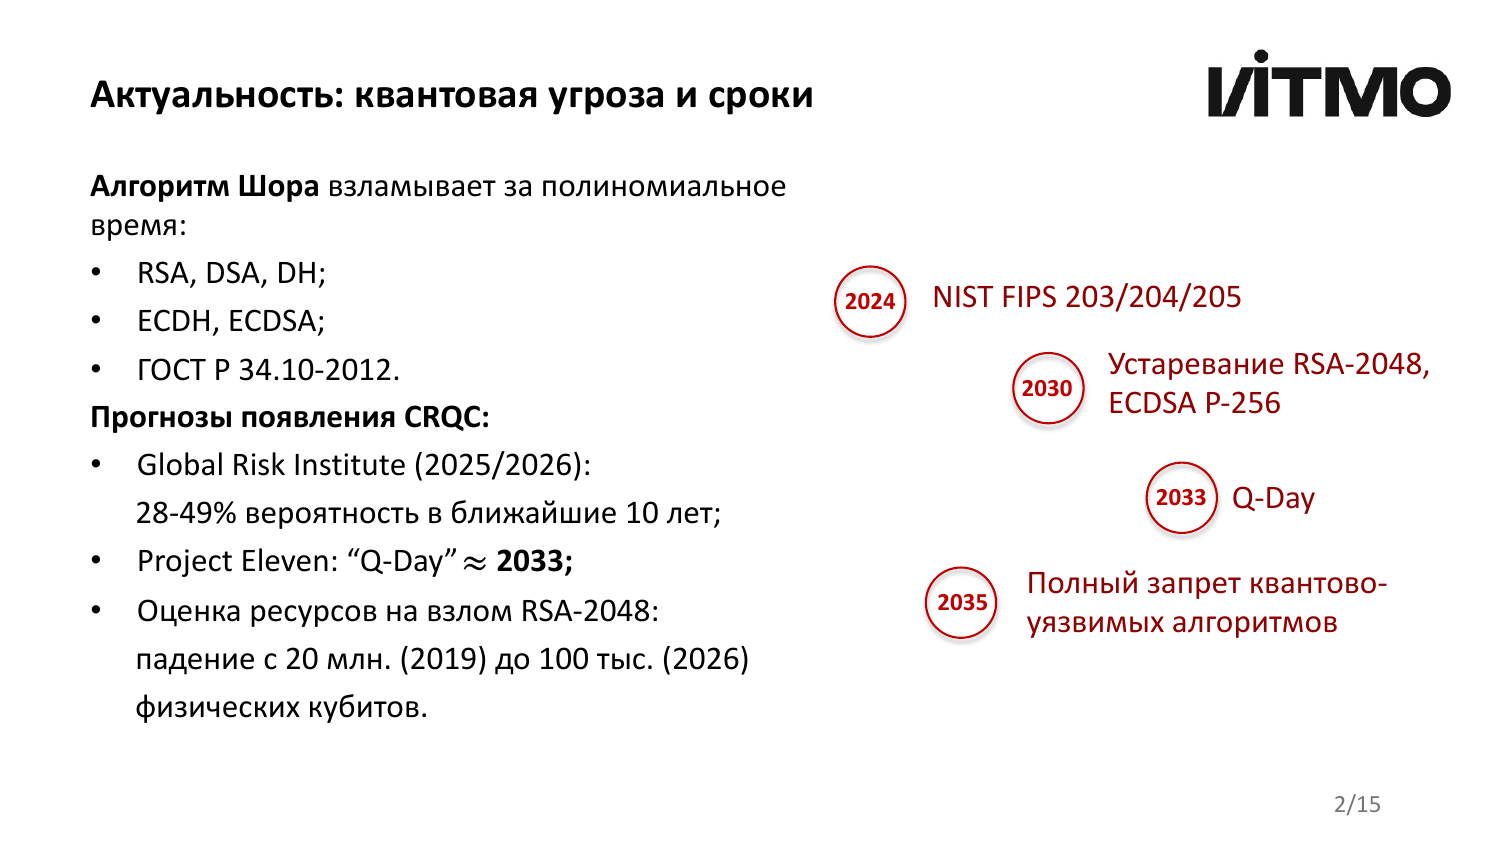
\includegraphics[width=\textwidth]{slides/slide-02.png}
    \caption{Слайд 2~-- Актуальность: квантовая угроза и сроки}
\end{figure}

\begin{figure}[H]
    \centering
    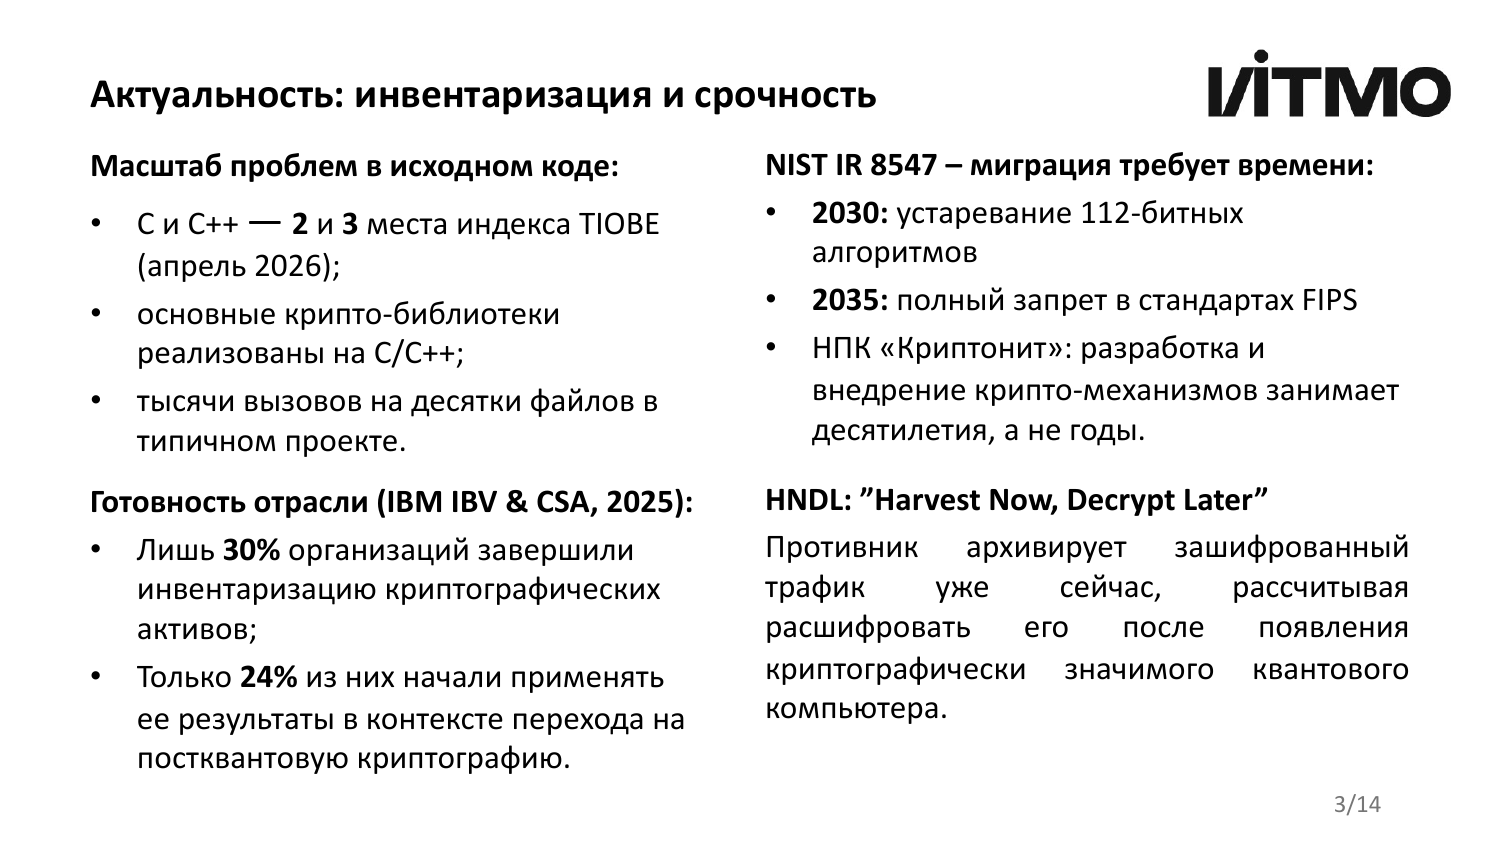
\includegraphics[width=\textwidth]{slides/slide-03.png}
    \caption{Слайд 3~-- Актуальность: инвентаризация и срочность}
\end{figure}

\begin{figure}[H]
    \centering
    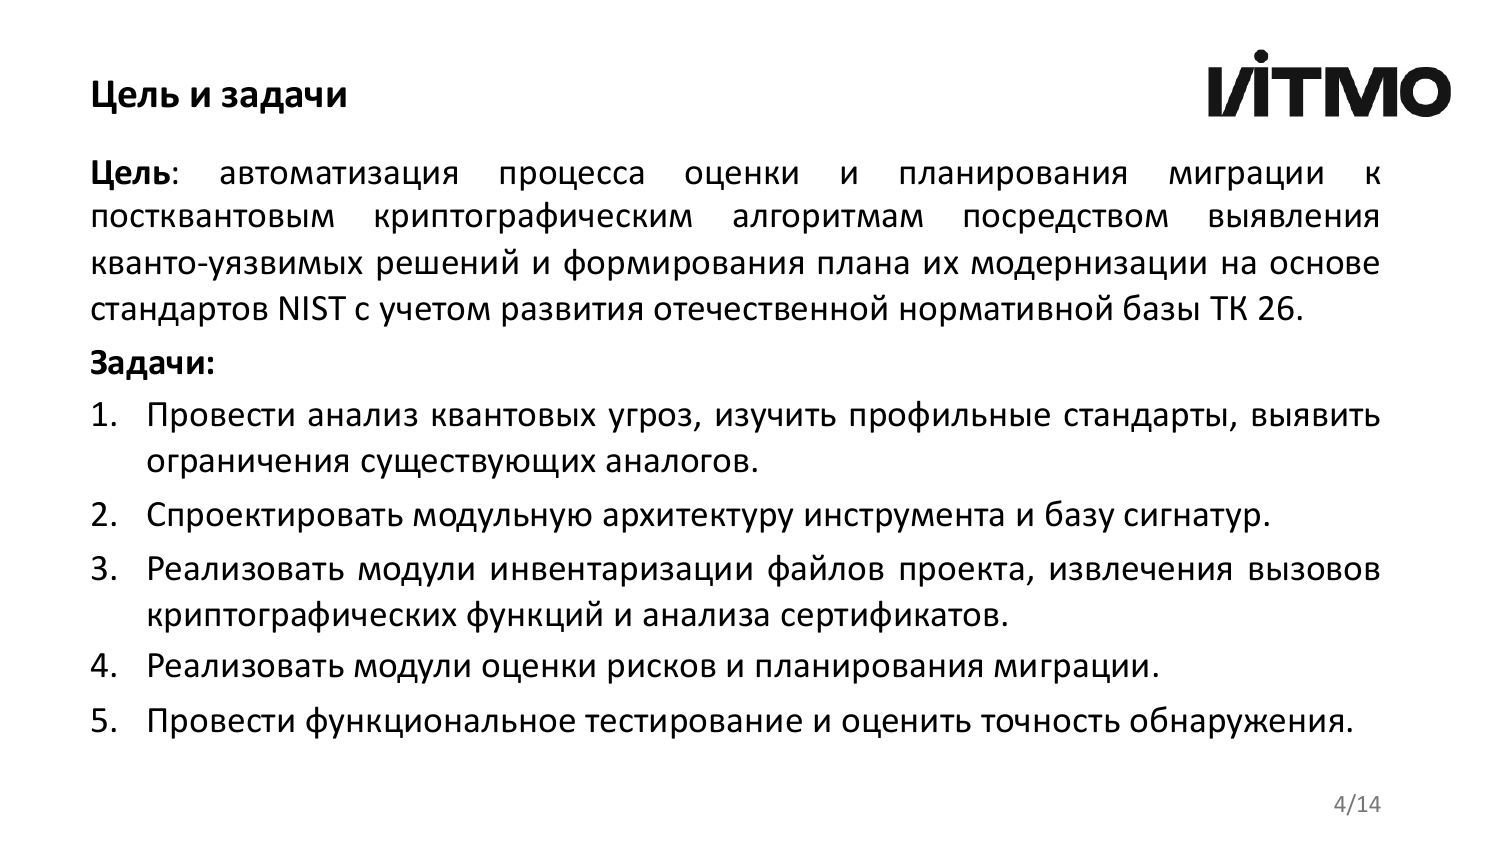
\includegraphics[width=\textwidth]{slides/slide-04.png}
    \caption{Слайд 4~-- Цель и задачи}
\end{figure}

\begin{figure}[H]
    \centering
    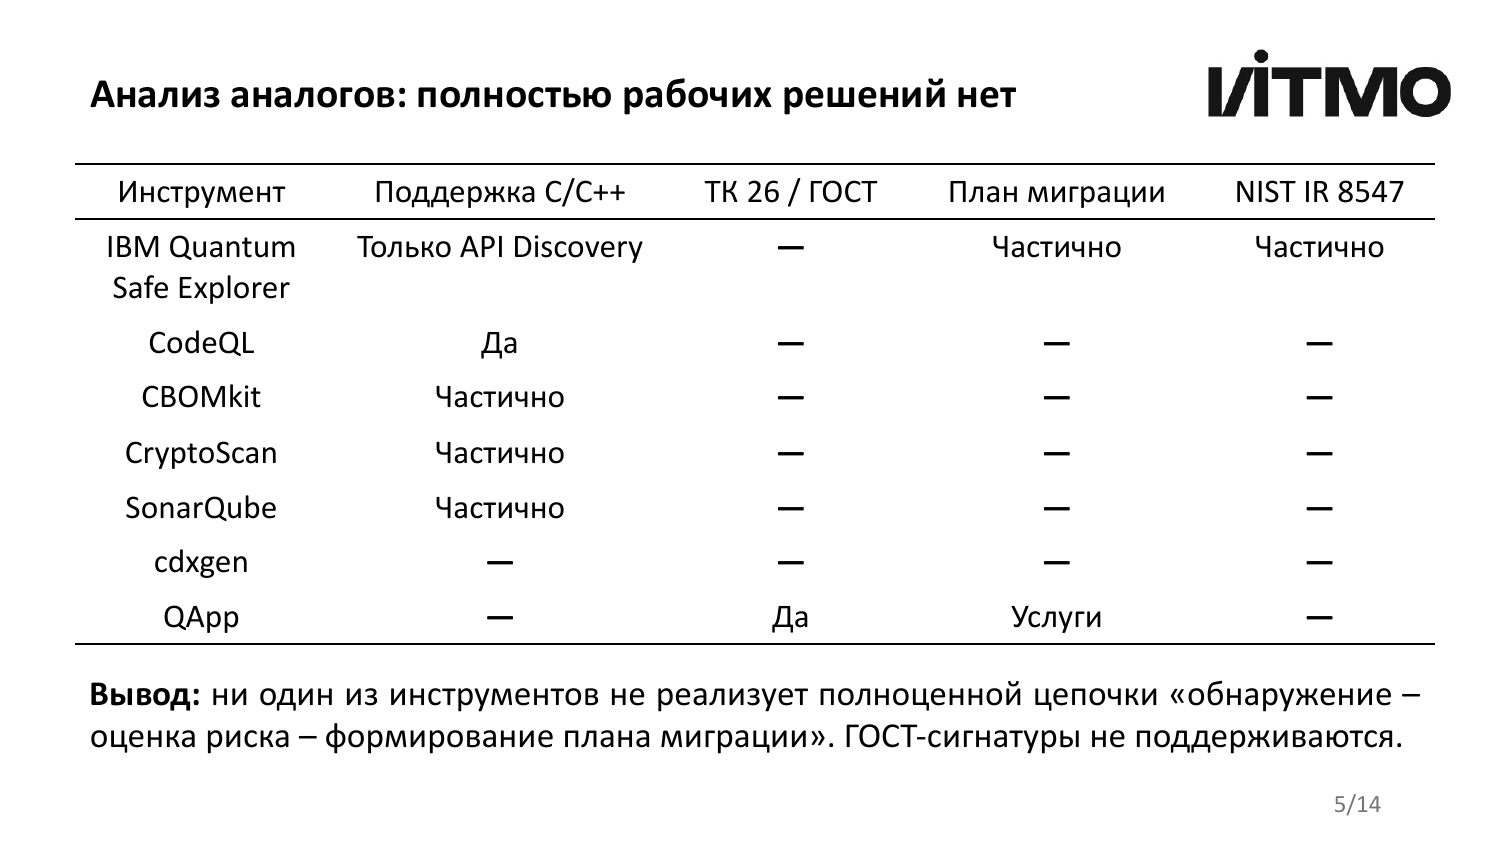
\includegraphics[width=\textwidth]{slides/slide-05.png}
    \caption{Слайд 5~-- Анализ аналогов}
\end{figure}

\begin{figure}[H]
    \centering
    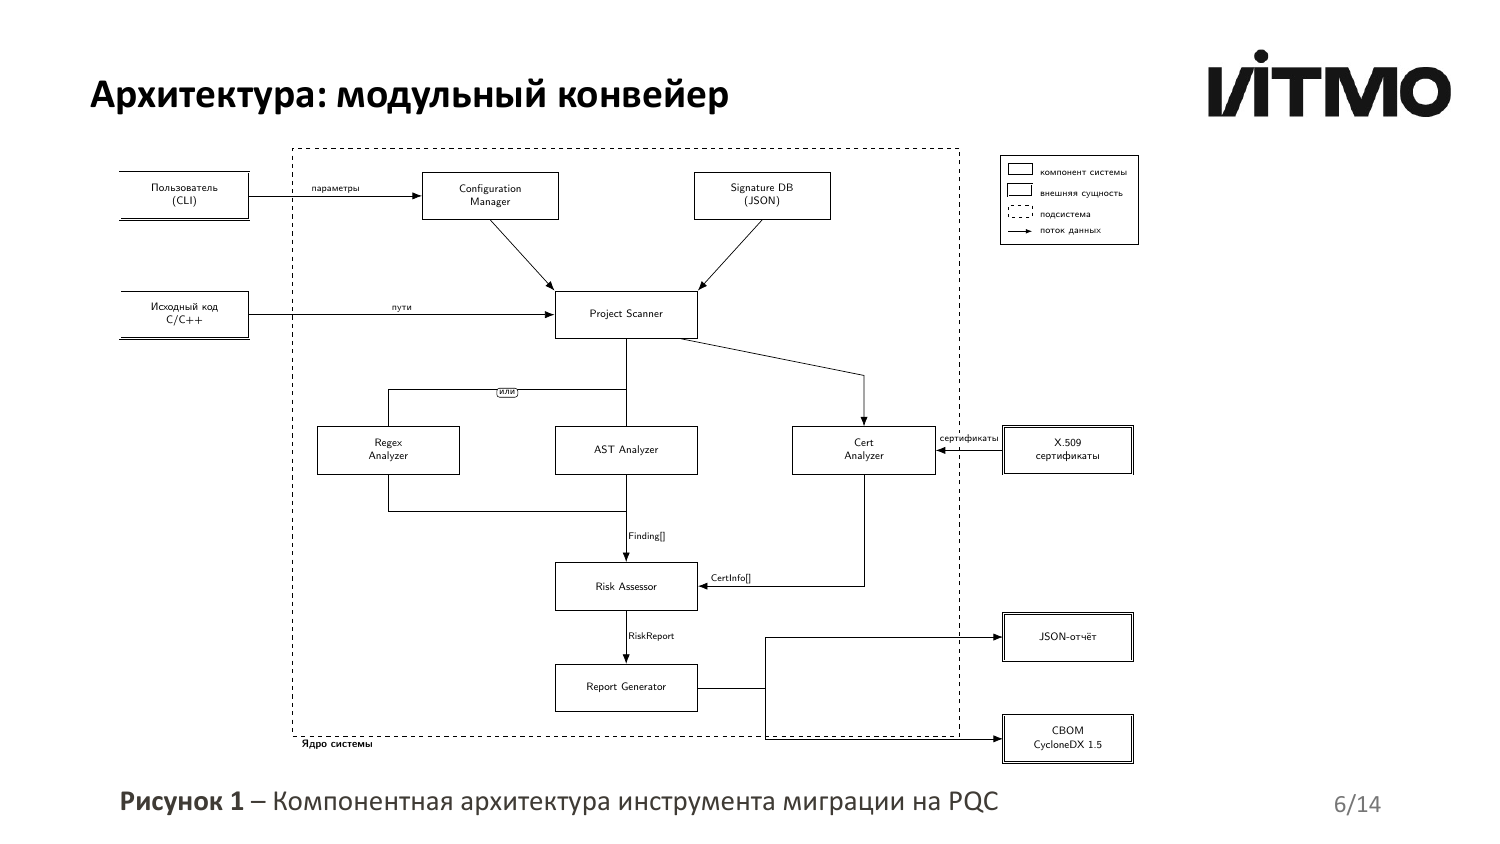
\includegraphics[width=\textwidth]{slides/slide-06.png}
    \caption{Слайд 6~-- Архитектура: модульный конвейер}
\end{figure}

\begin{figure}[H]
    \centering
    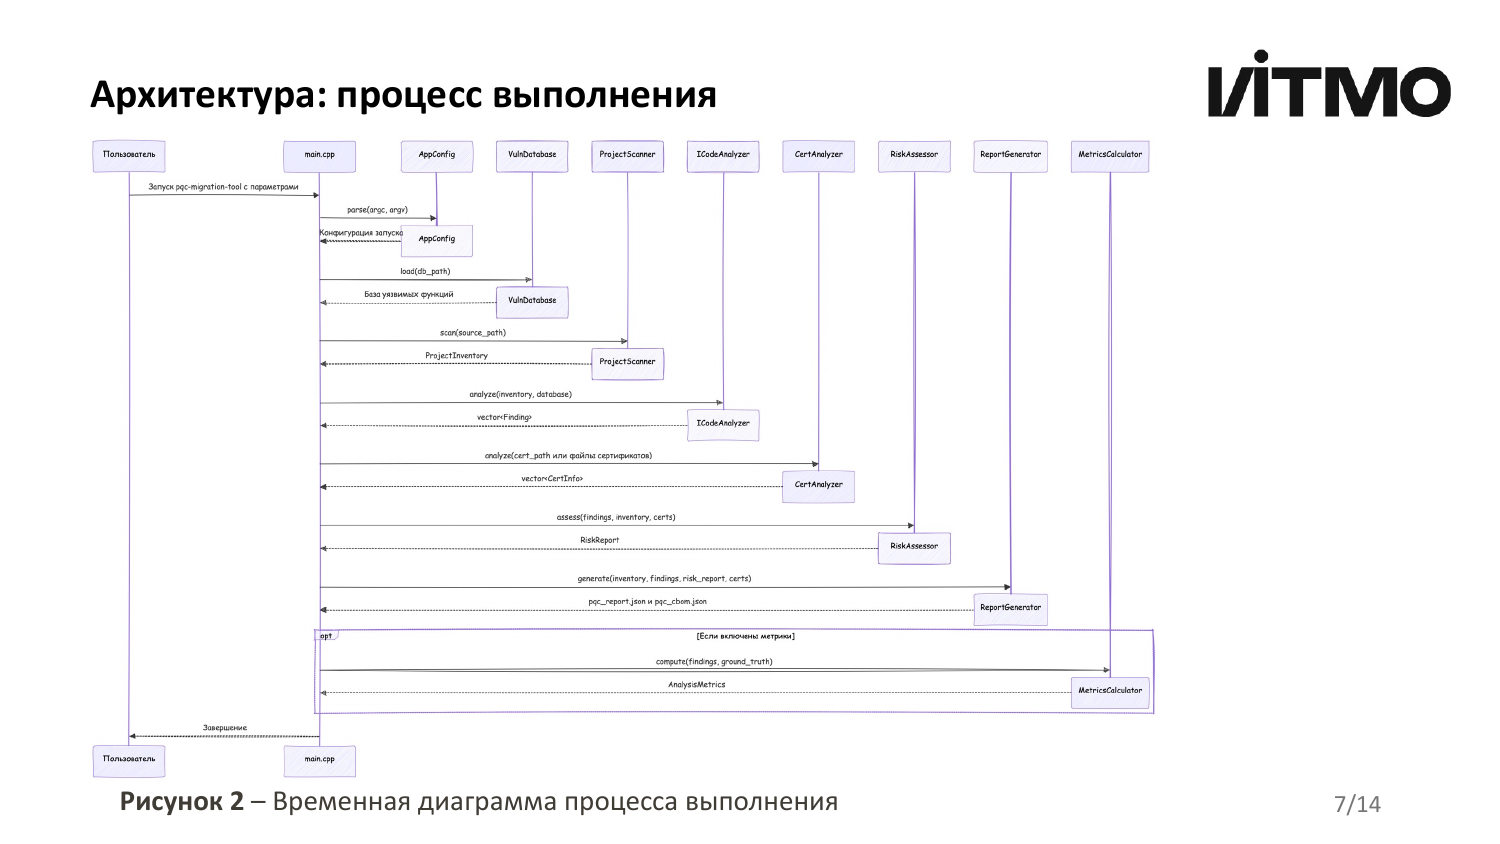
\includegraphics[width=\textwidth]{slides/slide-07.png}
    \caption{Слайд 7~-- Архитектура: процесс выполнения}
\end{figure}

\begin{figure}[H]
    \centering
    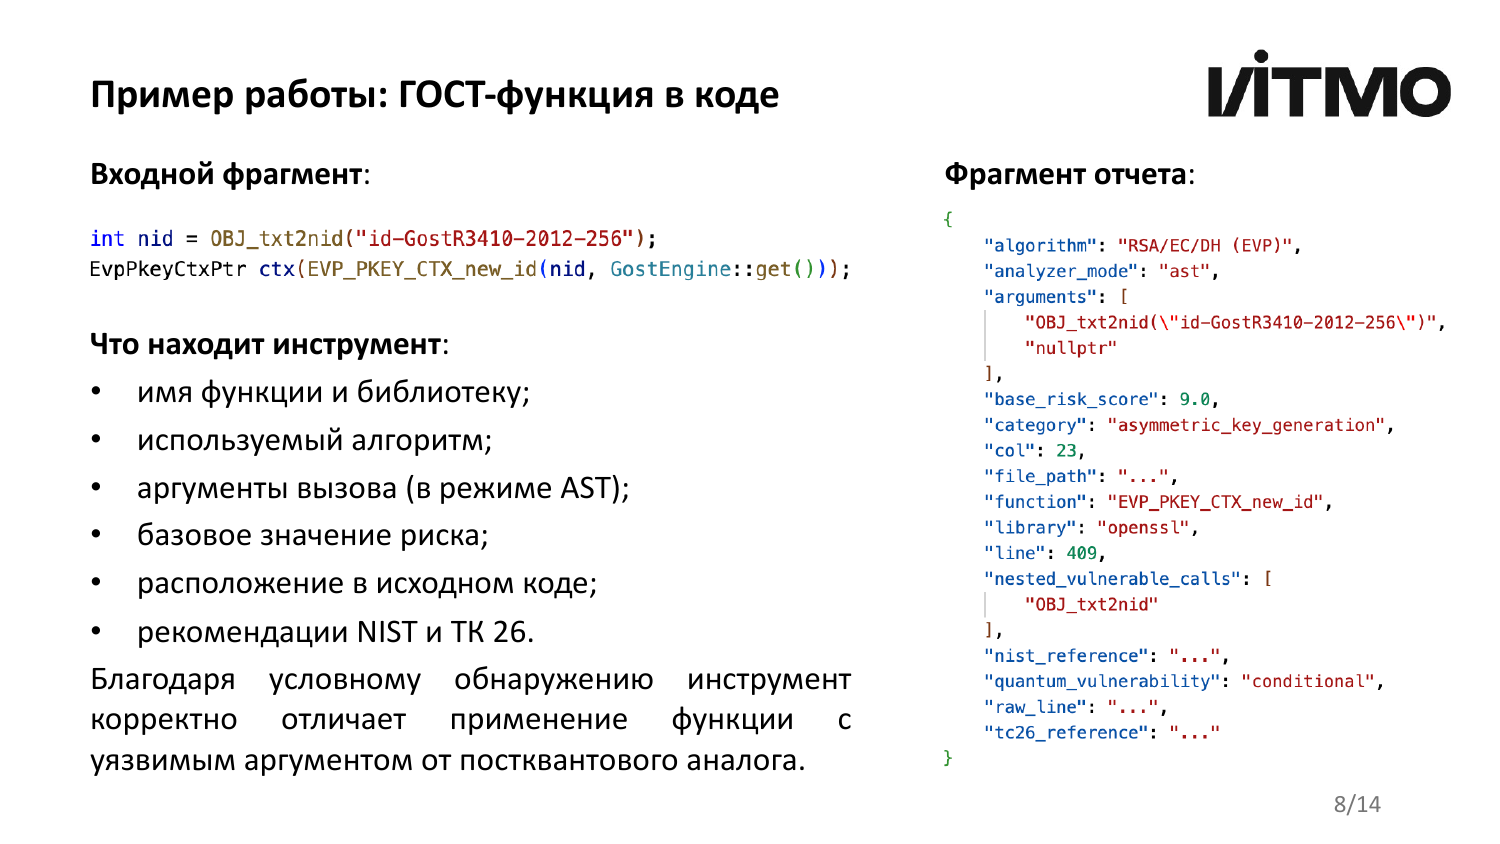
\includegraphics[width=\textwidth]{slides/slide-08.png}
    \caption{Слайд 8~-- Пример работы: ГОСТ-функция в коде}
\end{figure}

\begin{figure}[H]
    \centering
    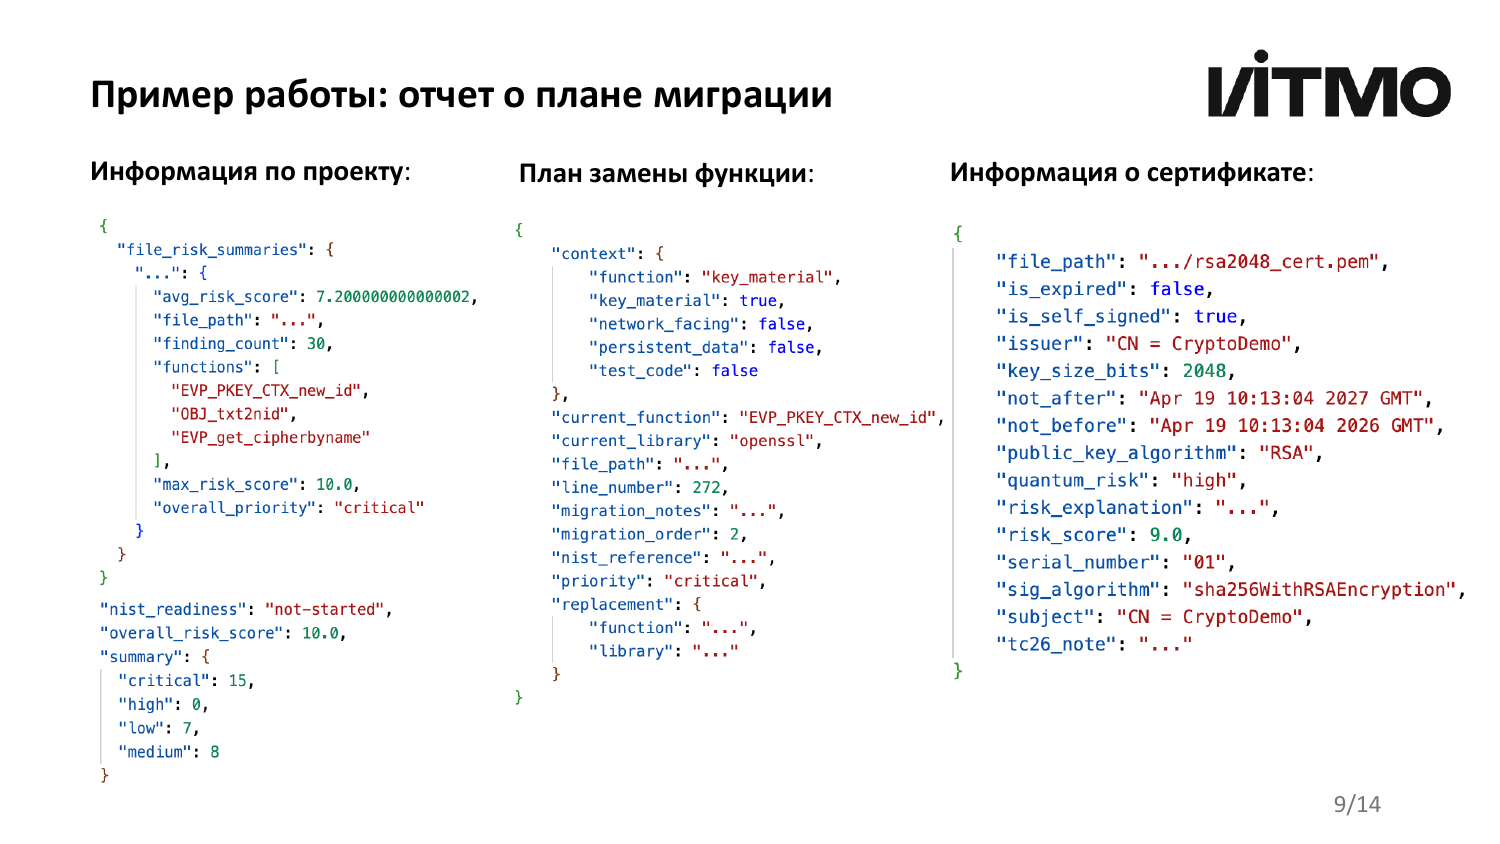
\includegraphics[width=\textwidth]{slides/slide-09.png}
    \caption{Слайд 9~-- Пример работы: отчёт о плане миграции}
\end{figure}

\begin{figure}[H]
    \centering
    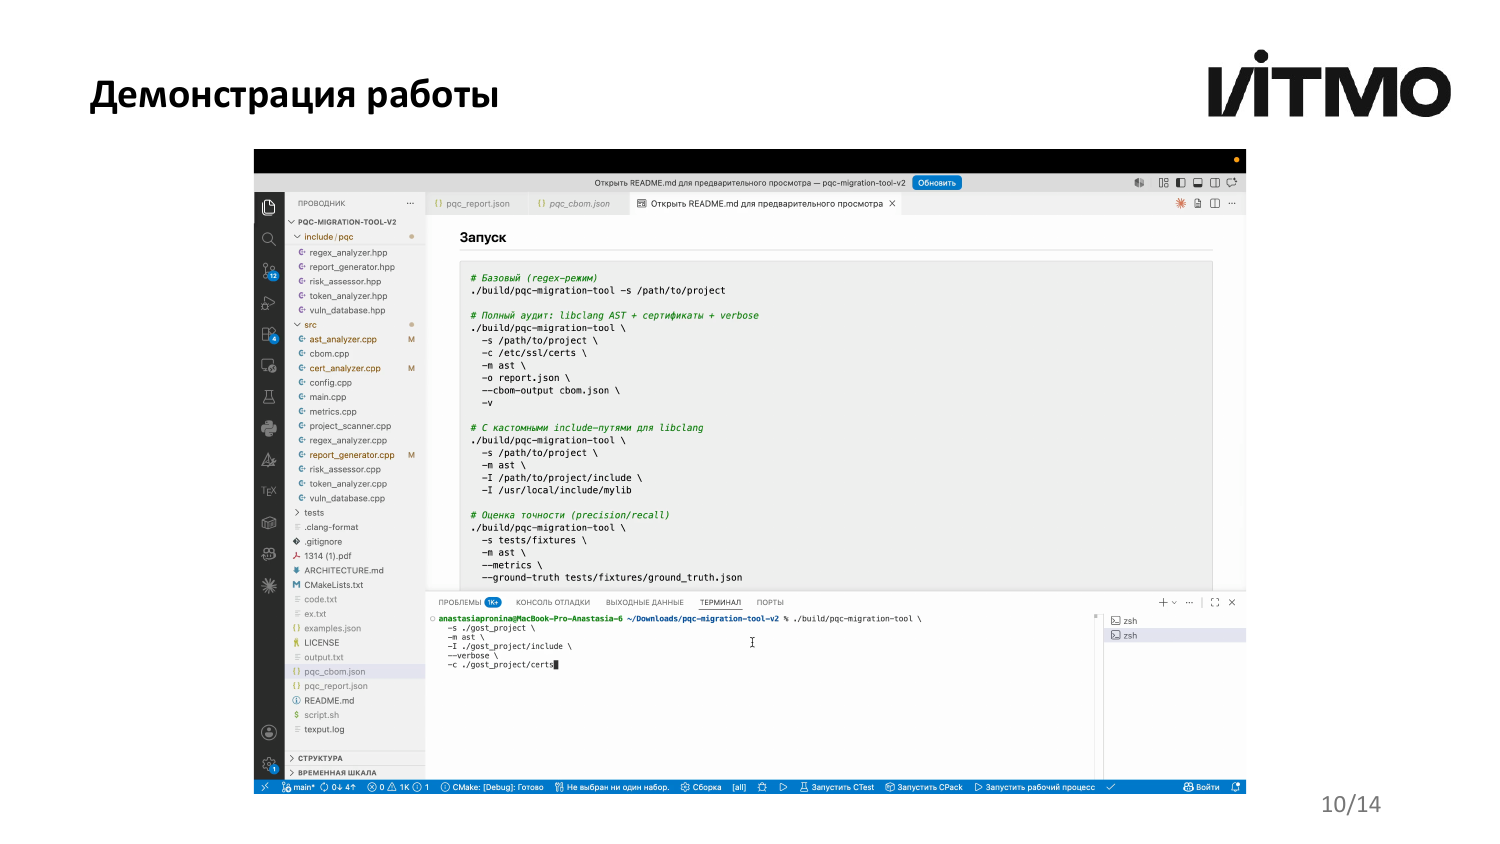
\includegraphics[width=\textwidth]{slides/slide-10.png}
    \caption{Слайд 10~-- Демонстрация работы}
\end{figure}

\begin{figure}[H]
    \centering
    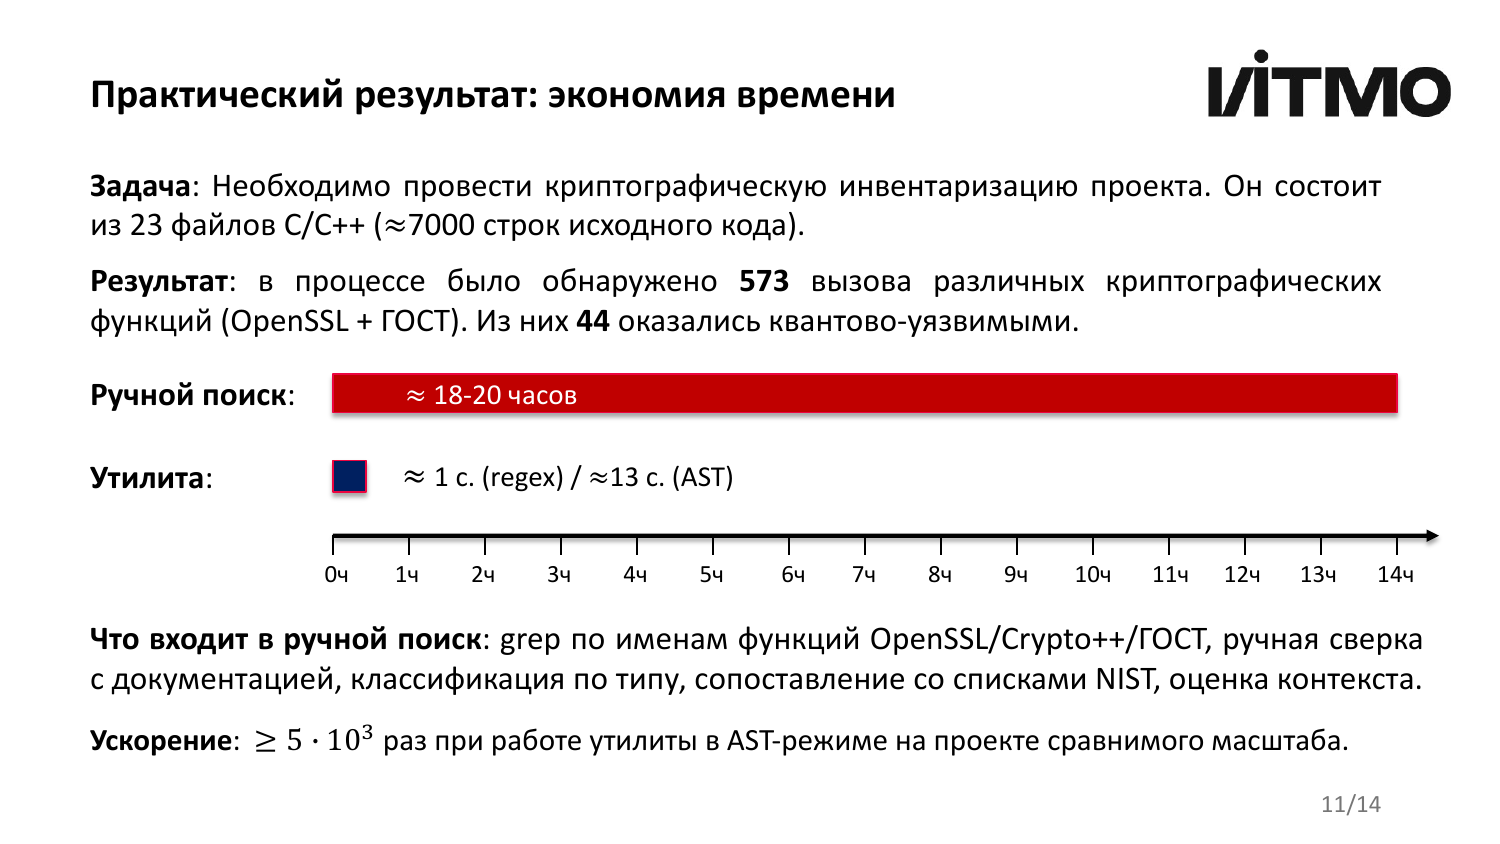
\includegraphics[width=\textwidth]{slides/slide-11.png}
    \caption{Слайд 11~-- Практический результат: экономия времени}
\end{figure}

\begin{figure}[H]
    \centering
    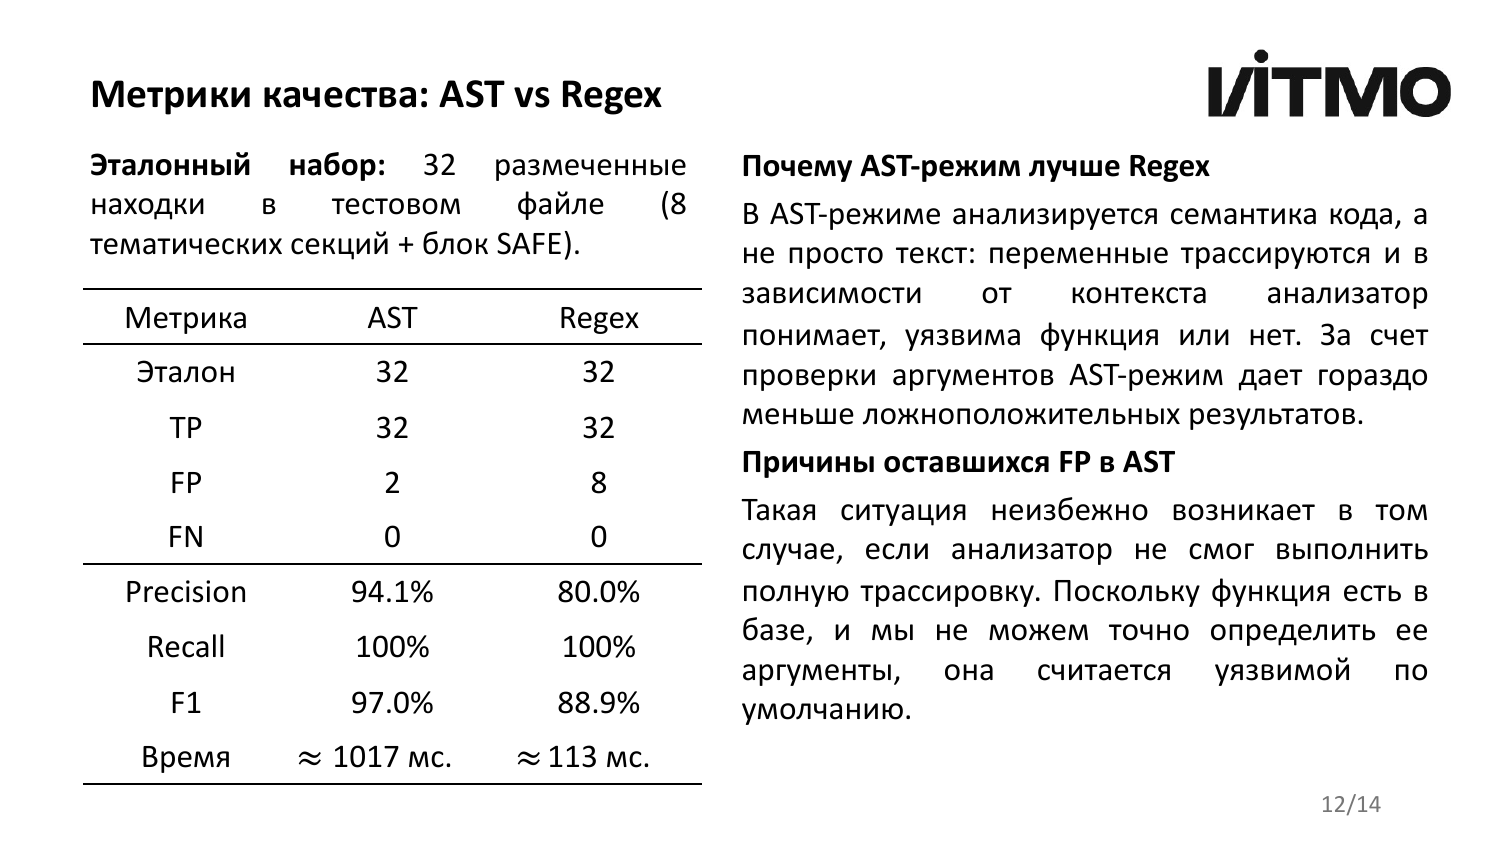
\includegraphics[width=\textwidth]{slides/slide-12.png}
    \caption{Слайд 12~-- Метрики качества: AST vs Regex}
\end{figure}

\begin{figure}[H]
    \centering
    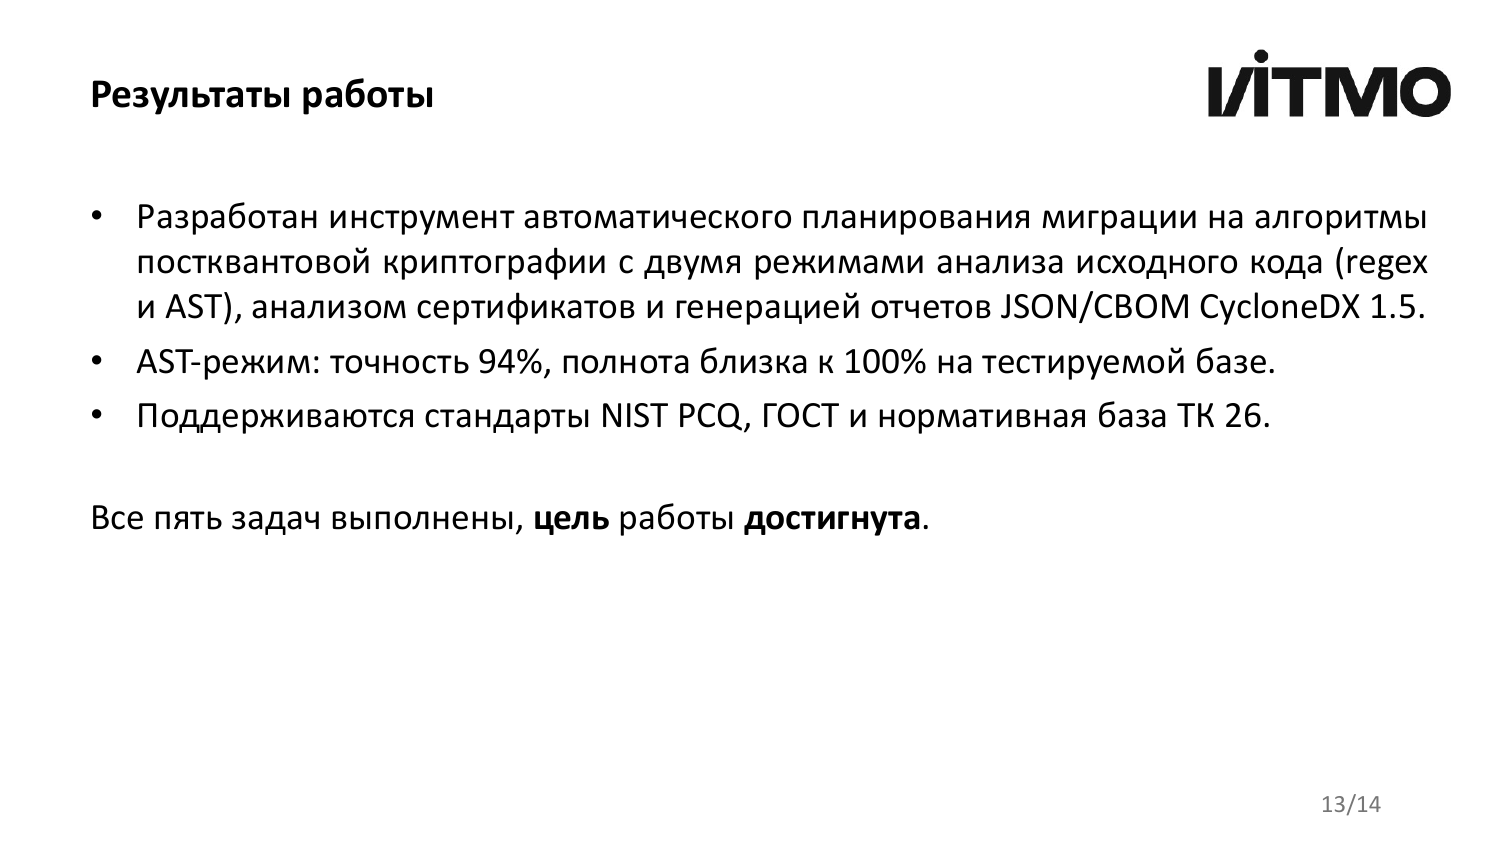
\includegraphics[width=\textwidth]{slides/slide-13.png}
    \caption{Слайд 13~-- Результаты работы}
\end{figure}

\begin{figure}[H]
    \centering
    
\includegraphics[width=\textwidth]{slides/slide-14.png}
    \caption{Слайд 14~-- Благодарность и ссылка на репозиторий}
\end{figure}

\end{document}
